\section{Token Tree Verifier}
\label{sec:verification}

\if 0 
\begin{figure}
    \centering
    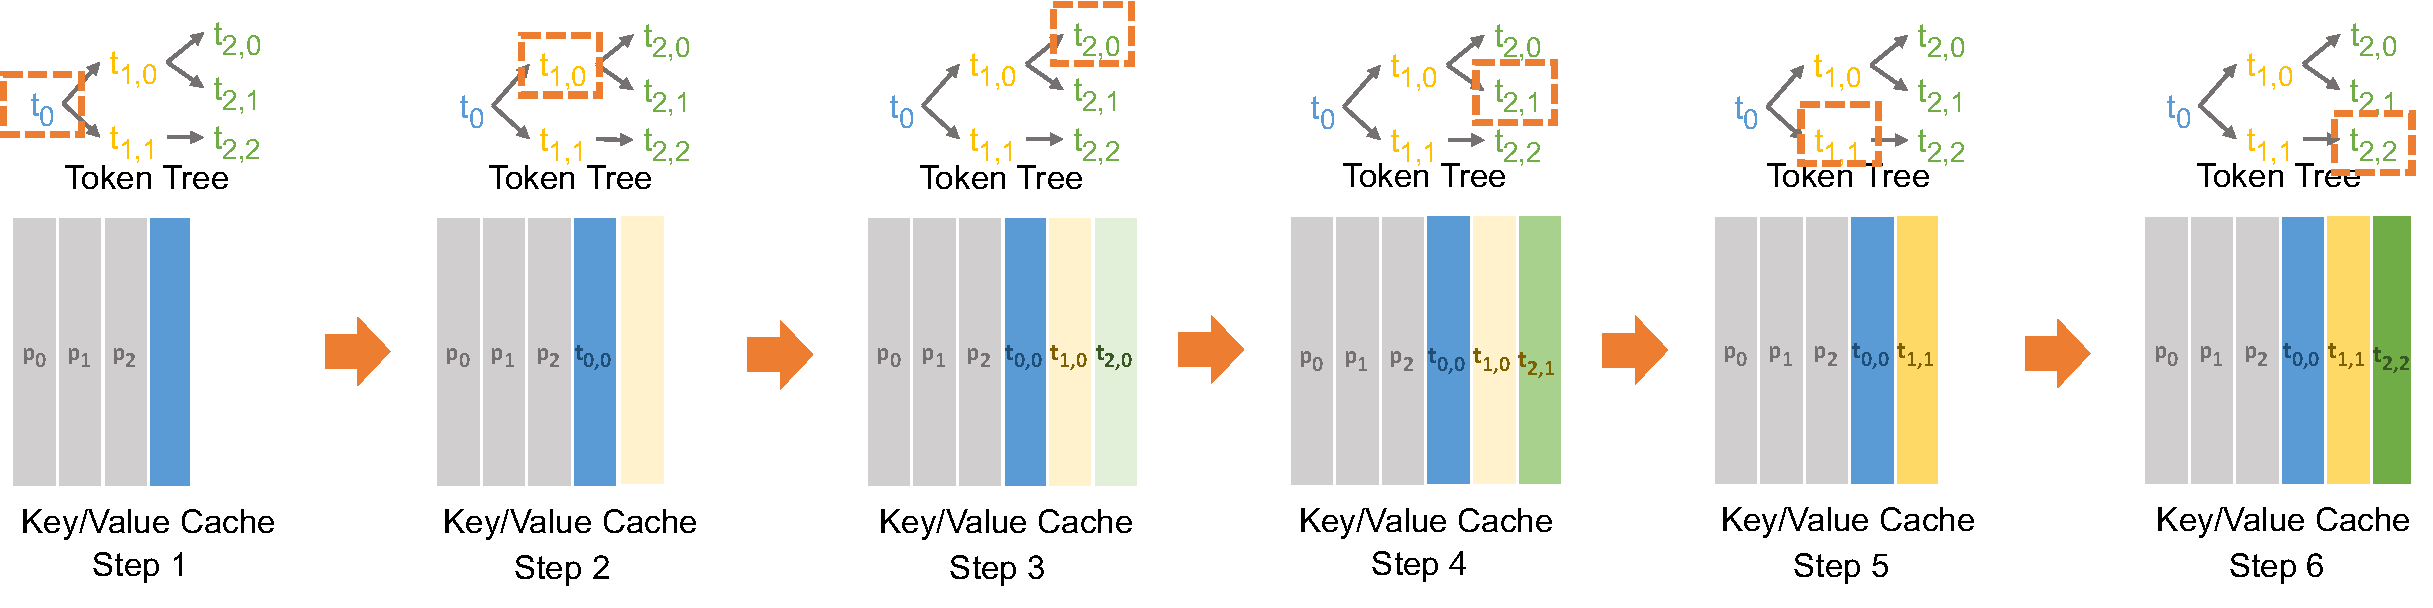
\includegraphics[scale=0.33]{figs/kv_cache_v3.pdf}
    \caption{\Sys's depth-first search mechanism to traverse a token tree.\XM{Working on this figure (Done, To be replaced)}}
    \label{fig:kv_cache}
\end{figure}
\fi

\begin{figure}
    \centering
    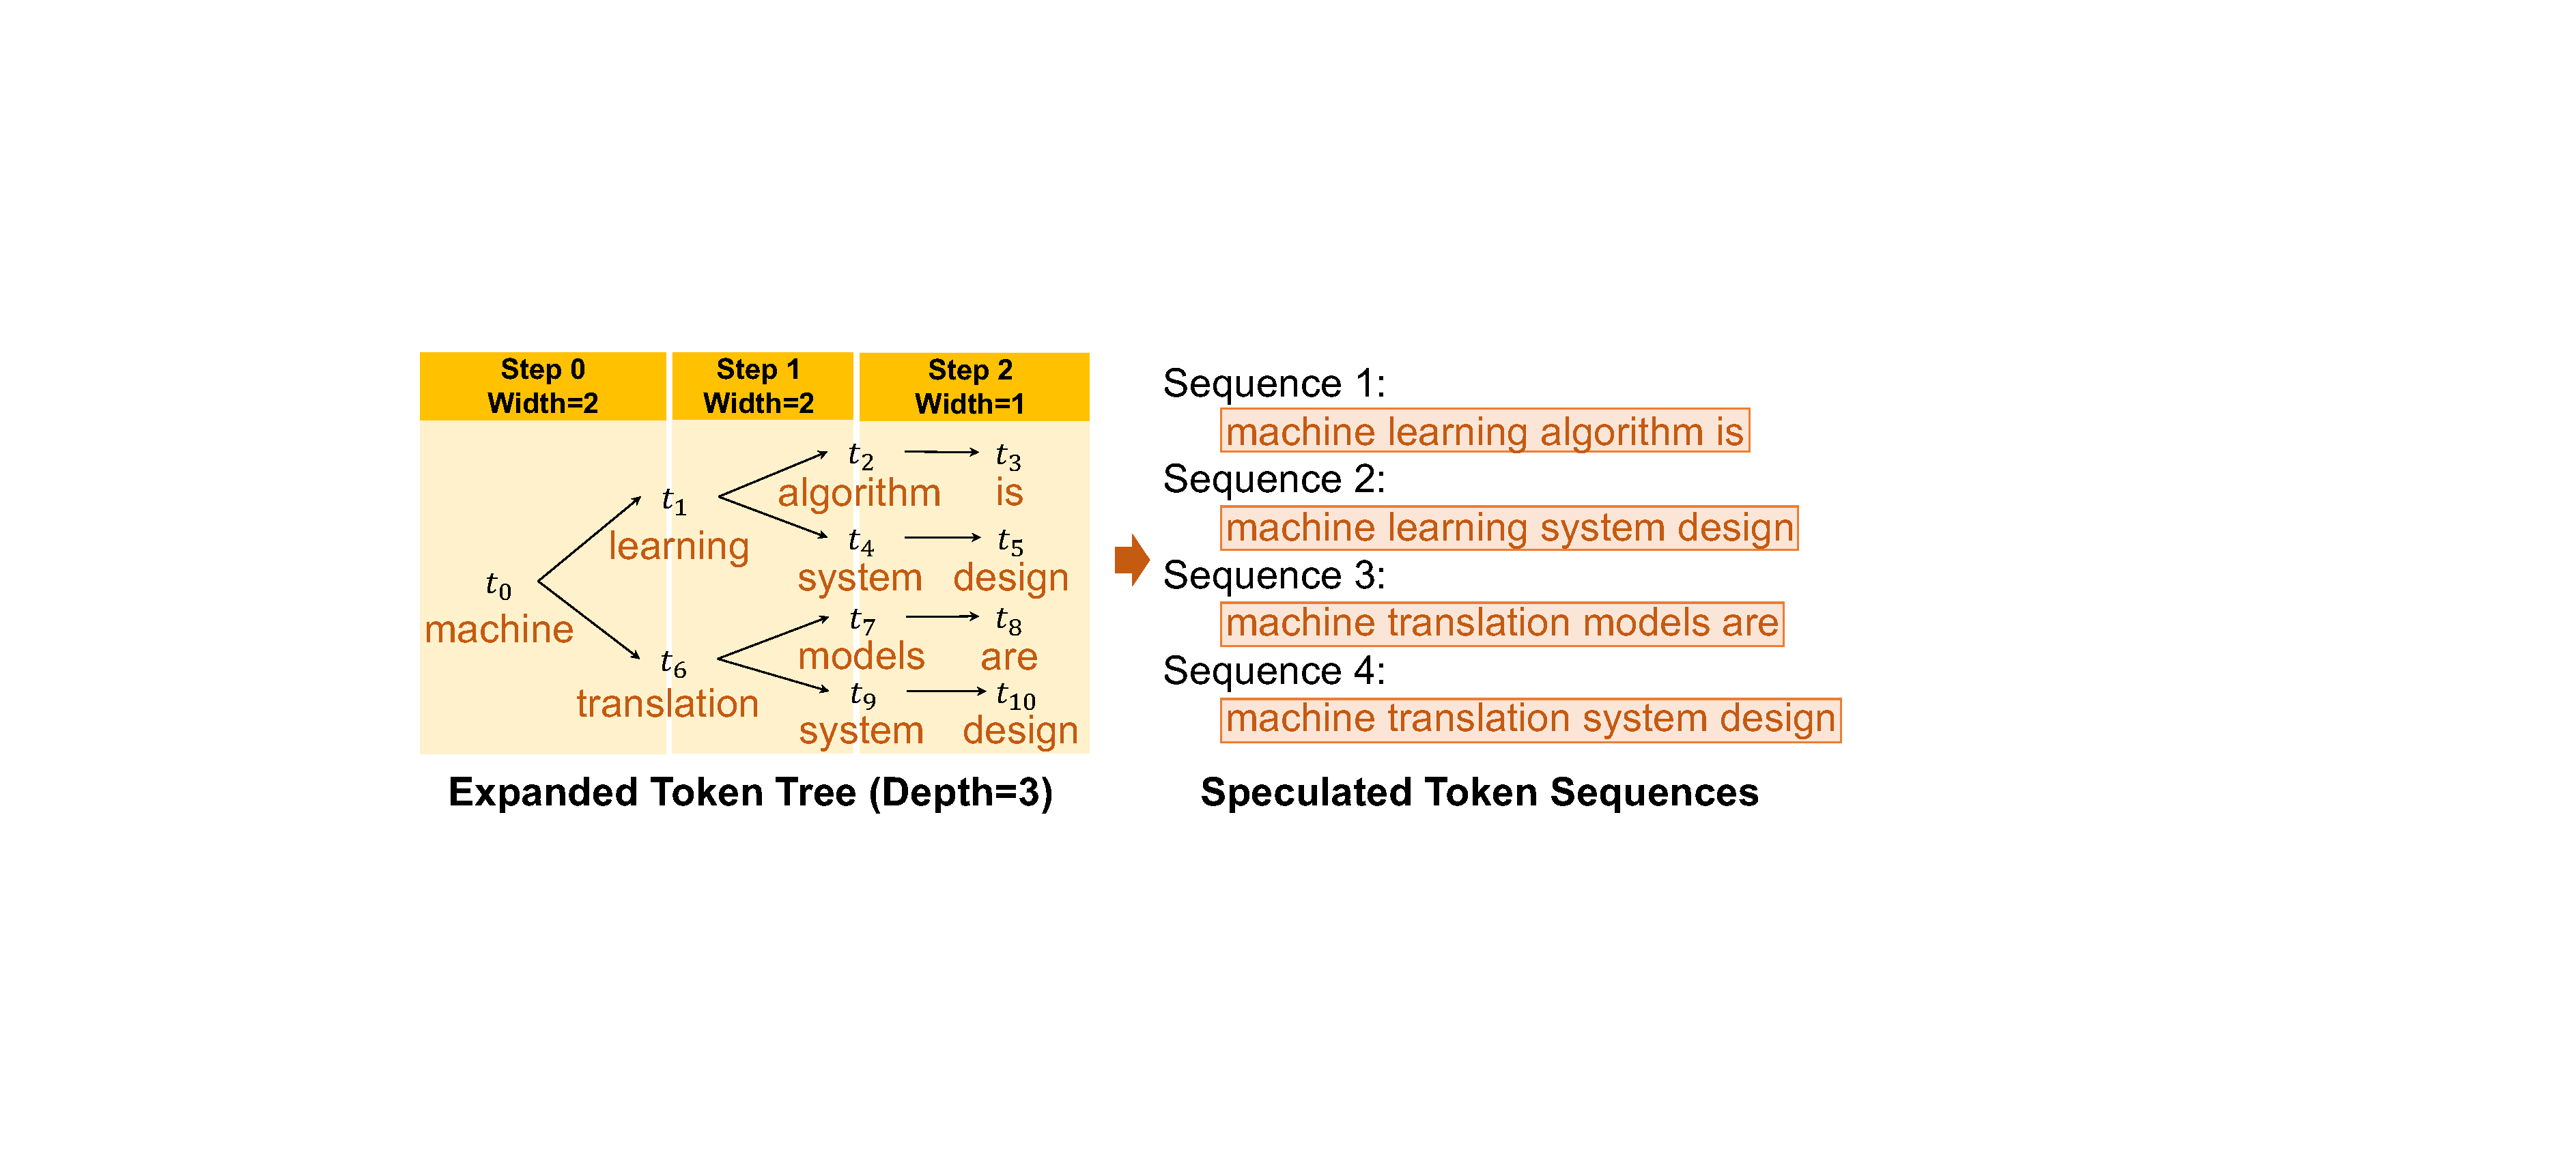
\includegraphics[width=\linewidth]{rebuttal_figs/token_tree3.pdf}
    \caption{\rev{Illustration of token tree expansion.}}
    % \ZJ{Fonts too small. Consider increasing the font size if possible.}
%     \caption{
% Merging three sequences of tokens (left) into a token tree (right), whose node each identifies a token sequence. For example, node $t_4$ represents a token sequence $[t_0, t_1, t_3, t_4]$ that translates to ``machine learning system design''.
% \XM{Working on this}}
    \label{fig:token_tree_merge}
\end{figure}

This section introduces \sys's {\em token tree verifier}, which takes as input a token tree generated by the speculator and verifies the correctness of its tokens against an LLM's output.
%
A key idea behind the design of \Sys is {\em simultaneously} verifying all sequences of a token tree against the original LLM's output by making a {\em single} pass over the LLM's parameters.
%%%
This functionality allows \Sys to opportunistically decode {\em multiple} tokens (instead of a single token in incremental decoding), resulting in reduced memory accesses to the LLM's parameters.
%%%
A challenge \Sys must address in token tree verification is efficiently computing the attention scores for {\em all} sequences of a token tree.
%%%
To this end, we introduce {\em tree attention}, which generalizes the attention mechanism~\cite{vaswani2017attention} from sequence to tree structure.
In addition, we develop a {\em tree-based parallel decoding} mechanism that can decode {\em all} tokens in a token tree in parallel.
%\Sys performs {\em tree attention}, a fast and cheap approach to performing Transformer-based attention computation for a token tree, and a number of important system-level optimizations to address this challenge.

\S\ref{subsec:tree_attention} and \S\ref{subsec:optimization} describe tree attention and tree-based parallel decoding. 
\S\ref{subsec:verification} introduces the mechanism to verify a token tree against the LLM's output.
%\Cref{subsec:verification} introduces the mechanism \Sys uses to verify a token tree against an LLM, and \Cref{subsec:optimization} presents \Sys's optimizations to accelerate token tree verification.

\if 0
\ZJ{TO BE REMOVED <---}
\begin{definition}[Token Tree]
A token tree $\m{N}$ is a tree structure, where each node $u \in \m{N}$ is labelled with a token $t_u$, and $p_u$ represents $u$'s parent node in the token tree. 
For each node $u$, $S_u$ represents a sequence of tokens identified by concatenating $S_{p_u}$ and $\{t_u\}$\footnote{For the root node $r$, $S_r$ represents the token sequence $\{t_r\}$.}.
\end{definition}

\Sys uses a {\em token tree} to store the results generated by the learning-based speculator. Specifically, \Sys receives multiple token sequences generated by different SSMs, each of which can be considered as a token tree (with linear tree structure), and merges them into a single token tree.

\begin{definition}[Token Tree Merge]
$\m{M}$ is the tree merge of $m$ token trees $\{\m{N}_i\}$ ($1\leq i \leq m$) if and only if $\forall 1\leq i \leq m, \forall u \in \m{N}_i, \exists v \in \m{M}$ such that $S_v = S_u$ and vice versa.
\end{definition}

Intuitively, each token tree represents a set of token sequences. Merging multiple token trees produces a new tree that includes all token sequences of the original trees.
For example, \Cref{fig:token_tree_merge} shows the token tree derived by merging three sequences of tokens.
Each token sequence is identified by a node in the merged token tree.
%and performs tree merge to produce a speculated token tree. Each token sequence can be considered as a special token tree. For $m$ input token trees $\{\m{N}_i\}$ ($1 \leq i \leq m$), $N$ is the output of 
\ZJ{--->TO BE REMOVED}
\fi 

\subsection{Tree Attention}
\label{subsec:tree_attention}
Transformer-based language models use the attention mechanism to reason about sequential information~\cite{vaswani2017attention}.
LLMs generally use decoder-only, multi-head self-attention, which takes a single input tensor $X$ and computes an output tensor $O$ via scaled multiplicative formulations as follows.
\begin{eqnarray}
    Q_i = X \times W_i^Q, & K_i = X \times W_i^K, \\
    V_i = X \times W_i^V, & A_i = \frac{(Q_i \times K_i^T)}{\sqrt{d}}, \\
    H_i = \textrm{softmax}\big(\textrm{mask}(A_i)\big) V_i, & O = (H_1, ...,H_h) W^O 
    \label{eqn2}
\end{eqnarray}
where $Q_i$, $K_i$, and $V_i$ denote the query, key, and value tensors of the $i$-th attention head ($1\leq i \leq h$), $W_i^Q$, $W_i^K$, and $W_i^V$ are the corresponding weight matrices. 
$A_i$ is an $l\times l$ matrix that represents the attention scores between different tokens in the input sequence, where $l$ is the sequence length. To preserve causality when generating tokens (i.e., a token in the sequence should not affect the hidden states of any preceding tokens), the following causal mask function is applied:
\begin{equation}
    \textrm{mask}(A)_{jk} =     \begin{cases}
    A_{jk} & j \geq k\\
    - \infty & j < k 
    \end{cases}.
\end{equation}
Intuitively, when computing the attention output of the $j$-th token in the sequence, all subsequent tokens should have an attention score of $-\infty$ to indicate that the subsequent tokens will not affect the attention output of the $j$-th token\footnote{Note that we use $-\infty$ (instead of 0) to guarantee that the softmax's output is 0 for these positions.}. 
%%%
In Equation~\ref{eqn2}, $H_i$ represents the output of the $i$-th attention head, and $W_O$ is a weight matrix used for computing the final output of the attention layer.

Note that the attention mechanism described above applies only to a sequence of tokens. We generalize the attention mechanism to arbitrary tree structures.
%For each node $u$ in a token tree, its tree attention is defined as the output of computing original attention on $S_u$ (i.e., the token sequence represented by $u$). 

\begin{definition}[Tree Attention]
For a token tree $\m{N}$ and an arbitrary node $u \in \m{N}$, its tree attention is defined as the output of computing the original Transformer-based sequence attention on $S_u$ (i.e., the token sequence represented by $u$):
\begin{equation}
    \textproc{TreeAttention}(u) = \textproc{Attention}(S_u) \forall u \in \m{N}
\end{equation}
\end{definition}
For a given set of token sequences, since each sequence $S$ is covered by a node of the merged token tree, performing tree attention on the token tree allows \Sys to obtain the attention output for {\em all} token sequences. 
% Note that the semantic of \Sys's tree attention is different from prior tree-structured attention work~\cite{Nguyen2020}, which we discuss in \Cref{sec:related}.


\subsection{Tree-based Parallel Decoding}
\label{subsec:optimization}

\begin{figure*}
    \centering
    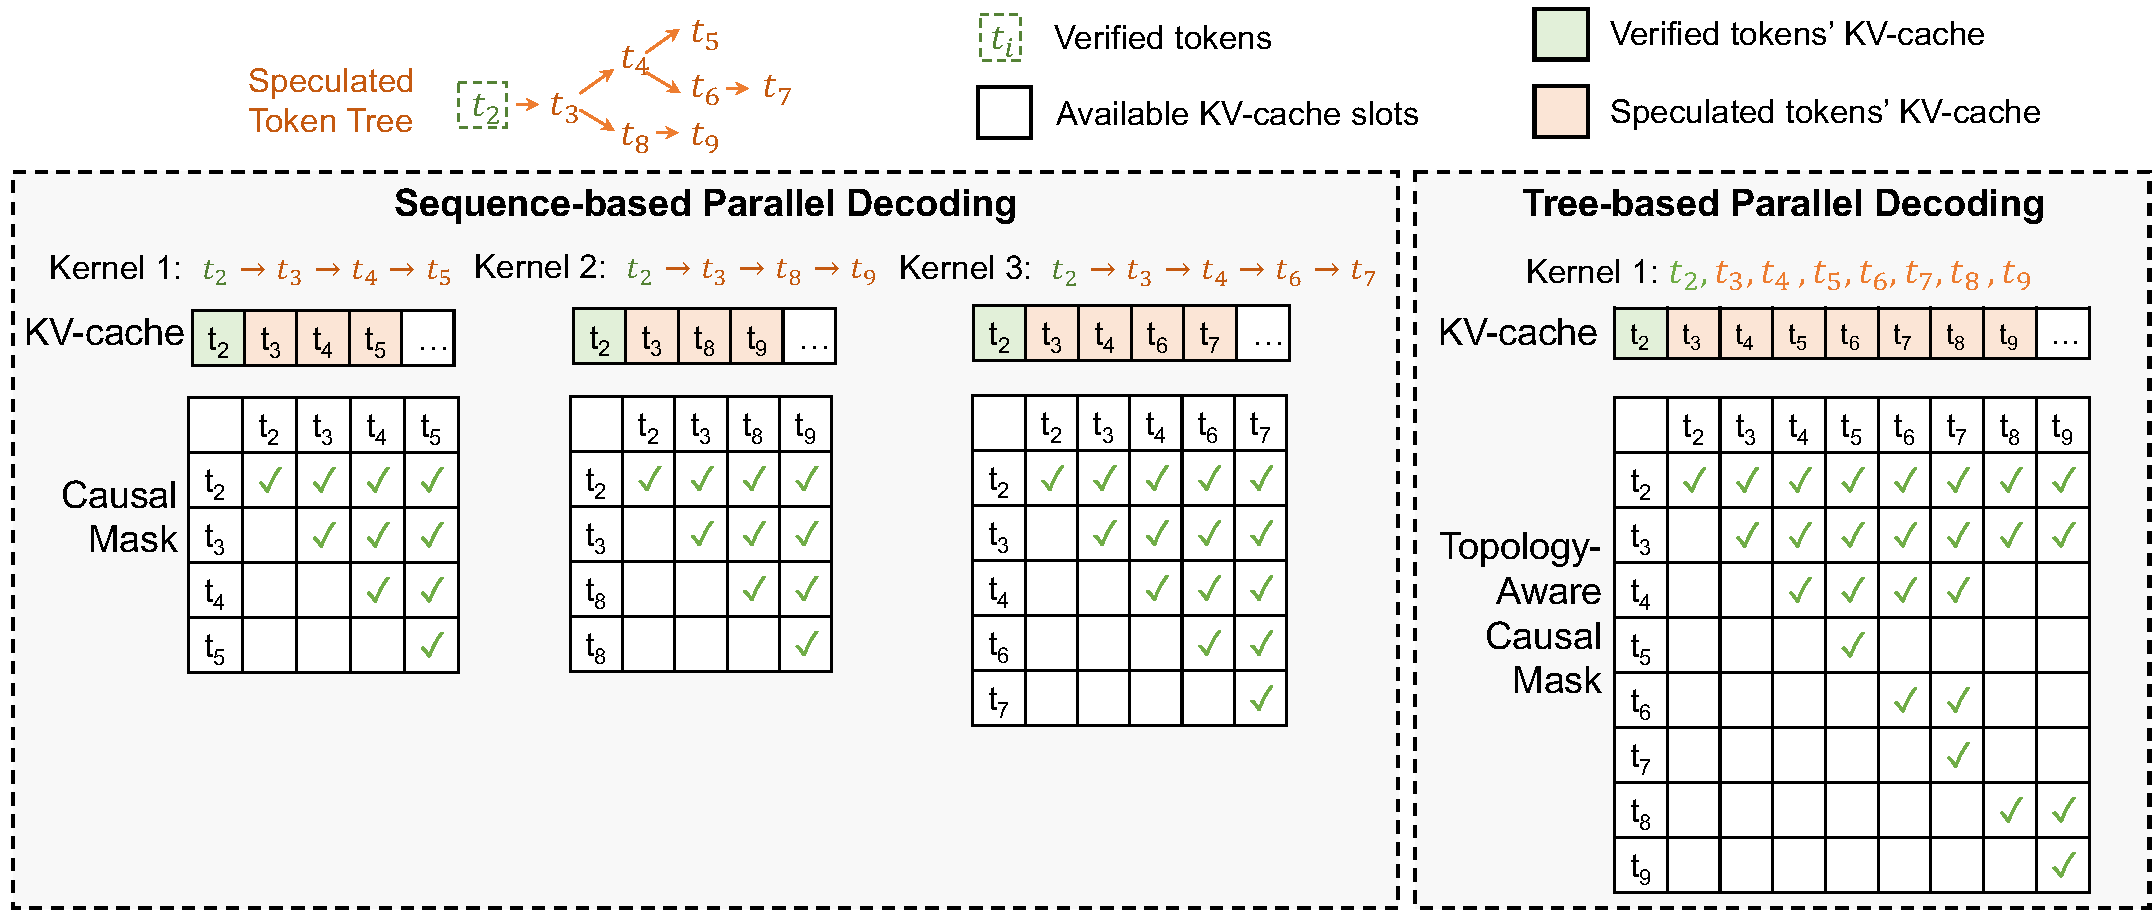
\includegraphics[width=0.9\textwidth]{figs/new_kv_cache2.pdf}
    \caption{Comparing \Sys's tree-based parallel decoding with existing sequence-based decoding.}
    \label{fig:kv_cache}
\end{figure*}

This section describes \sys's {\em tree-based parallel decoding} mechanism for computing tree attention for {\em all} tokens in a token tree {\em in parallel}.
A key challenge \Sys must address in computing tree attention is managing {\em key-value cache}. 
%%%
In particular, the attention mechanism of Transformer~\cite{vaswani2017attention} requires accessing the keys and values of all preceding tokens to compute the attention output of each new token, as shown in Equation~\ref{eqn2}.
%%%
To avoid recomputing these keys and values, today's LLM inference systems generally cache the keys and values of all tokens for reuse in future iterations, since the causal relation guarantees that a token's key and value remain unchanged in subsequent iterations (i.e., $\rm{mask(A)_{jk}} = -\infty$ for any $j < k$).
%%% 
However, when computing tree attention, different sequences in a token tree may include conflicting key-value caches. For example, for the speculated token tree in \Cref{fig:kv_cache}, two token sequences $(t_2, t_3, t_4, t_5)$ and $(t_2, t_3, t_8, t_9)$ have different keys and values for the third and fourth positions.

A straightforward approach to supporting key-value cache is employing the sequence-based decoding of existing LLM inference systems and using a different key-value cache for each sequence of a token tree, as shown on the left of \Cref{fig:kv_cache}.
However, this approach is computationally very expensive and involves redundant computation, since two token sequences sharing a common prefix have the same attention outputs for the common prefix due to the causal mask in Equation~\ref{eqn2}.
In addition, launching one kernel for each token sequence introduces additional kernel launch overhead.

\Sys introduces two key techniques to realize tree-based parallel decoding.

\paragraph{Depth-first search to update key-value cache.} Instead of caching the keys and values for individual token sequences of a token tree, \Sys reuses the same key-value cache across all token sequences by leveraging a {\em depth-first search} mechanism to traverse the token tree, as shown in \Cref{fig:kv_cache}, where \Sys visits $t_2,t_3,...,t_9$ by following a depth-first order to traverse the token tree and update the shared key-value cache.
%%%
This approach allows \Sys to maintain the correct keys and values for all preceding tokens when computing the attention output of a new token.

\paragraph{Topology-aware causal mask.} A straightforward approach to computing tree attention is calculating the tree attention output for individual tokens by following the depth-first order described earlier. 
However, this approach would result in high GPU kernel launch overhead since each kernel only computes tree attention for one token sequence.
In addition, executing these kernels in parallel requires additional GPU memory to store their key-value caches separately due to cache conflict.
%%%
A key challenge that prevents \Sys from batching multiple tokens is that the attention computation for different tokens requires different key-value caches and therefore cannot be processed in parallel.

We introduce {\em topology-aware casual mask} to fuse tree attention computation of all tokens in a single kernel. 
To batch attention computation, \Sys uses a tree topology instead of the original sequence topology to store the keys and values of all tokens in a token tree in the key-value cache.
%the key-value cache of all speculated tokens of a token tree when computing attention scores.
For example, to compute tree attention for the speculated token tree shown in \Cref{fig:kv_cache}, \Sys takes both verified tokens (i.e., $t_2$) and all speculated tokens (i.e., $t_3,t_4,...,t_9$) as inputs.
This approach allows \Sys to fuse the attention computation into a single kernel but also results in attention scores that violate the causal dependency (e.g., $t_7$'s attention computation uses all previous tokens, including $t_5$ which is not in $t_7$'s token sequence).
To fix the attention scores for these pairs, \Sys updates the causal mask based on the token tree's topology.
This approach computes the exact same attention output as incremental decoding, while resulting in much fewer kernel launches compared to sequence-based decoding.

\if 0 

\section*{Old version}
This section describes \sys's {\em tree-based parallel decoding} algorithm for computing tree attention for {\em all} tokens in a token tree {\em in parallel}.
A straightforward approach to computing tree attention is directly computing the original sequence-based attention for all token sequences (i.e., $\textproc{Attention}(S_u$) for all $u\in\m{N}$).
However, this approach is computationally very expensive and involves redundant computation, since two token sequences sharing a common prefix have the same attention outputs for the common prefix due to the causal mask in Equation~\ref{eqn2}.

\paragraph{Depth-first search to update key-value cache.} As shown in Equation~\ref{eqn2}, the attention mechanism of Transformer~\cite{vaswani2017attention} requires accessing the keys and values of all preceding tokens to compute the attention output of each new token.
To avoid recomputing these keys and values, today's LLM inference systems generally cache the keys and values of all tokens for reuse in future iterations, since the causal relation guarantees that a token's key and value remain unchanged in subsequent iterations (i.e., $\rm{mask(A)_{jk}} = -\infty$ for any $k > j$).

A key challenge \Sys must address in verifying a token tree is that different sequences in the token tree may include conflicting key-value caches. For the speculated token tree at the top of \Cref{fig:kv_cache}, two token sequences $(t_2, t_3, t_4, t_5)$ and $(t_2, t_3, t_8, t_9)$ have different keys and values for the third and fourth positions.
%%%
A straightforward approach to supporting key-value cache is employing the sequence-based decoding of existing LLM inference systems and having a different key-value cache for each sequence of a token tree, as shown in the top-left of \Cref{fig:kv_cache}.
%%%
However, this approach requires multiple replicas of key-value caches for verifying different sequences and introduces redundant computations since sequences in a token tree may share common prefixes.

Instead of caching the keys and values for individual token sequences of a token tree, \Sys reuses the same key-value cache across all token sequences by leveraging a {\em depth-first search} mechanism to traverse the token tree, as shown in the top-right of \Cref{fig:kv_cache}, where the arrows indicate how the key-value cache is updated when decoding different tokens.
%%%
By following a depth-first order to traverse the token tree and update the shared key-value cache, \Sys is able to maintain the correct keys and values for all preceding tokens when computing the attention output of a new token. 

\paragraph{Tree-based parallel decoding.} Existing LLM inference systems use an incremental decoding approach that decodes a single token in each iteration during the generative phase. 
%%%
Therefore, a similar approach for computing tree attention is iteratively calculating the attention output for individual tokens in the token tree by following the depth-first order described earlier.
%using a depth-first order to traverse the token tree and computing the attention score for one token in each iteration.
%%%
However, this approach would result in high GPU kernel launch overhead since each kernel only computes tree attention for a single token.
%%%
A key challenge that prevents \Sys from batching multiple tokens is that the attention computation for different tokens requires different key-value caches and therefore cannot be processed in parallel.
For example, the token-based decoding in \Cref{fig:kv_cache} shows the key-value caches needed for each token.

\Sys uses a {\em tree-based parallel decoding} algorithm to opportunistically batch multiple tokens in a token tree. Specifically, \Sys leverages the causal mask of generative LLM inference and groups multiple tokens into a single kernel if each token is the subsequent token's parent.
%%%
For example, a depth-first search to traverse the token tree in \Cref{fig:kv_cache} is $(t_3, t_4, t_5, t_6, t_7, t_8, t_9)$. Instead of launching 7 individual kernels to compute the tree attention for these tokens, \Sys groups them into three kernels: $(t_3, t_4, t_5)$, $(t_6, t_7)$, and $(t_8, t_9)$, within each of which a token is a child of the previous token.
%%%
To batch attention computation, \Sys uses the key-value cache of the kernel's last token (i.e., $t_5$ for the first kernel), which results in attention scores that violate the causal dependency. \Sys then fixes the attention scores for these pairs.
%%%
This approach computes the exact same attention output as incremental decoding, while achieving much fewer kernel launches compared to the sequence and token-based decoding mechanism.
\fi 

%\paragraph{Committing tokens.}
%The depth-first order \Sys uses to traverse a token tree does not guarantee that \Sys stores correct key-value cache after the tree-based parallel decoding. 


\subsection{Token Verification}
\label{subsec:verification}

For a given speculated token tree $\m{N}$, 
%\Sys uses the tree attention mechanism described in \Cref{subsec:tree_attention} to compute an attention output for each node $u\in\m{N}$. 
%%%
%A key advantage of this approach is enabling \Sys to examine all tokens in parallel by visiting the LLM's parameters once.
%%%
\Sys uses tree-based parallel decoding (see \Cref{subsec:optimization}) to compute its tree attention and generate an output tensor $\m{O}$ that includes a token for each node $u\in\m{N}$.
%%%
Next, \Sys's {\em token tree verifier} examines the correctness of speculated tokens against the LLM. 
\Sys supports both greedy and stochastic sampling as shown in~\Cref{alg2}. 
%%%
\if 0
\textproc{Speculate} takes the current token sequence $\m{S}$ as an input and generates a speculated token tree $\m{N}$. 
% \Sys's use of an LLM is different from existing systems: the LLM takes a token tree $\m{N}$ as an input and generates a token $\m{O}(u)$ for each node $u \in \m{N}$.
The \textproc{TreeParallelDecode} function then generates all tokens in $\m{O}$ in a single LLM decoding step (see~\Cref{sec:verification}).
Finally, \textproc{VerifyGreedy} and \textproc{VerifyStochastic} examine the speculated token tree $\m{N}$ against the LLM's output $\m{O}$ and produces a sequence of verified tokens $\m{V}$ following greedy decoding or stochastic sampling respectively, which can be directly appended to the current token sequence $\m{S}$.
\fi
%%%
%Besides, \Sys further supports both greedy decoding and stochastic decoding as illustrated in~\Cref{fig:decodings} and described below.
\begin{figure}
    \centering
    %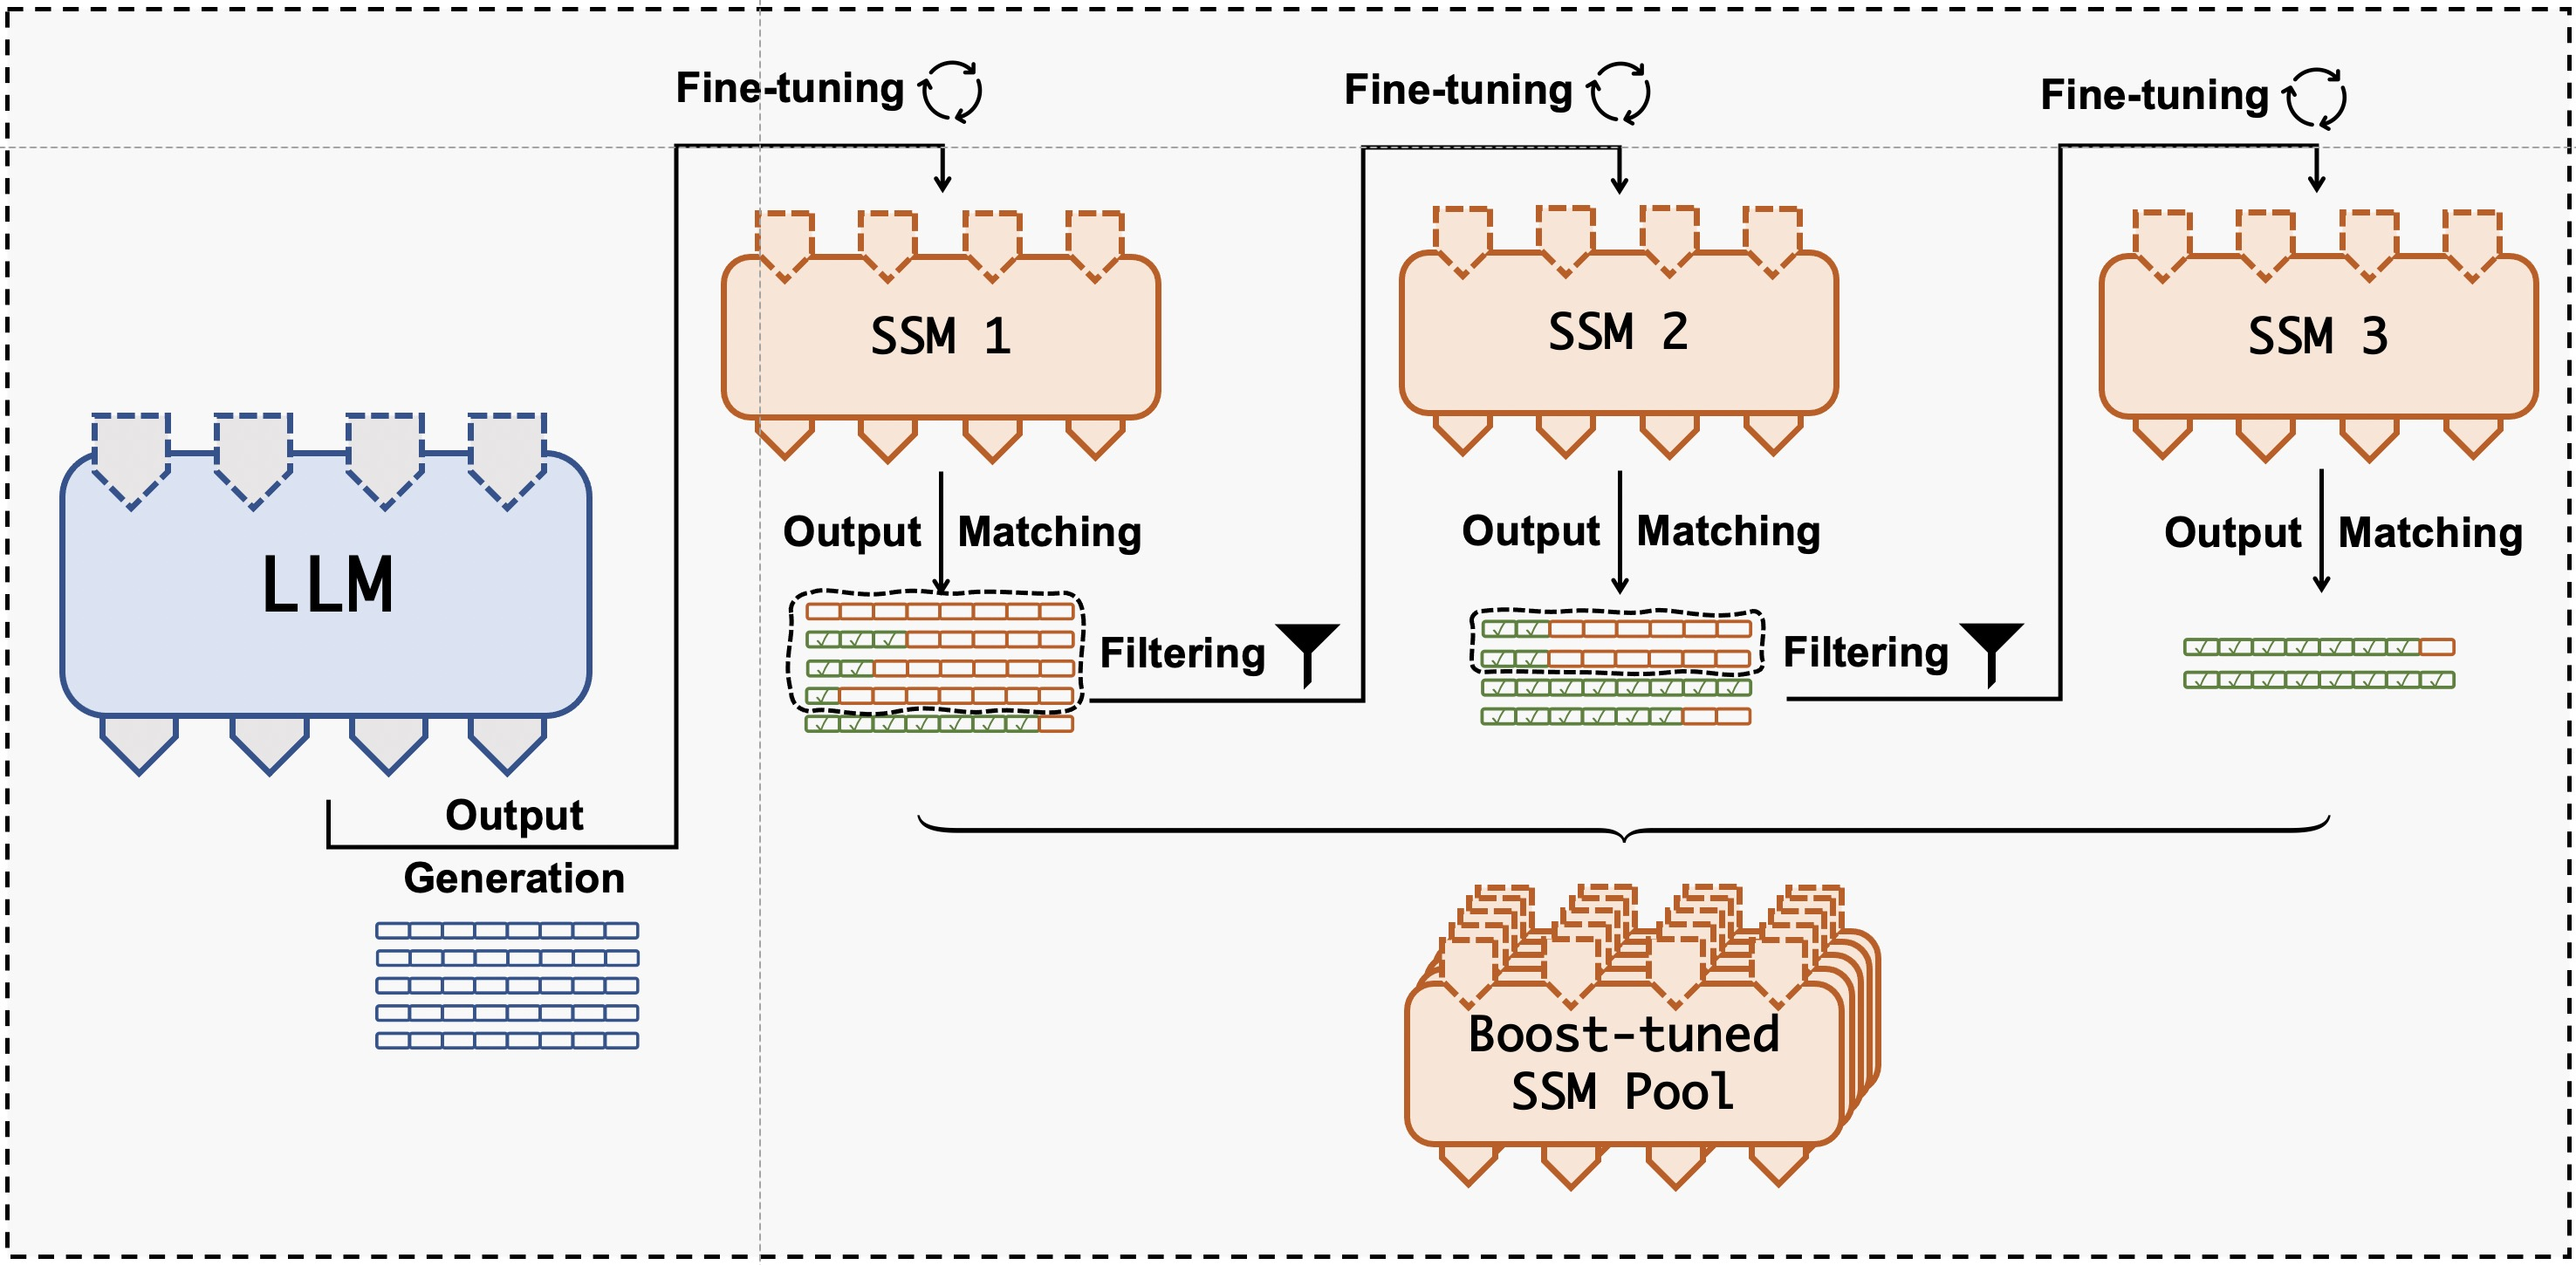
\includegraphics[scale=0.12]{figs/boost_tuning2.jpg}
    %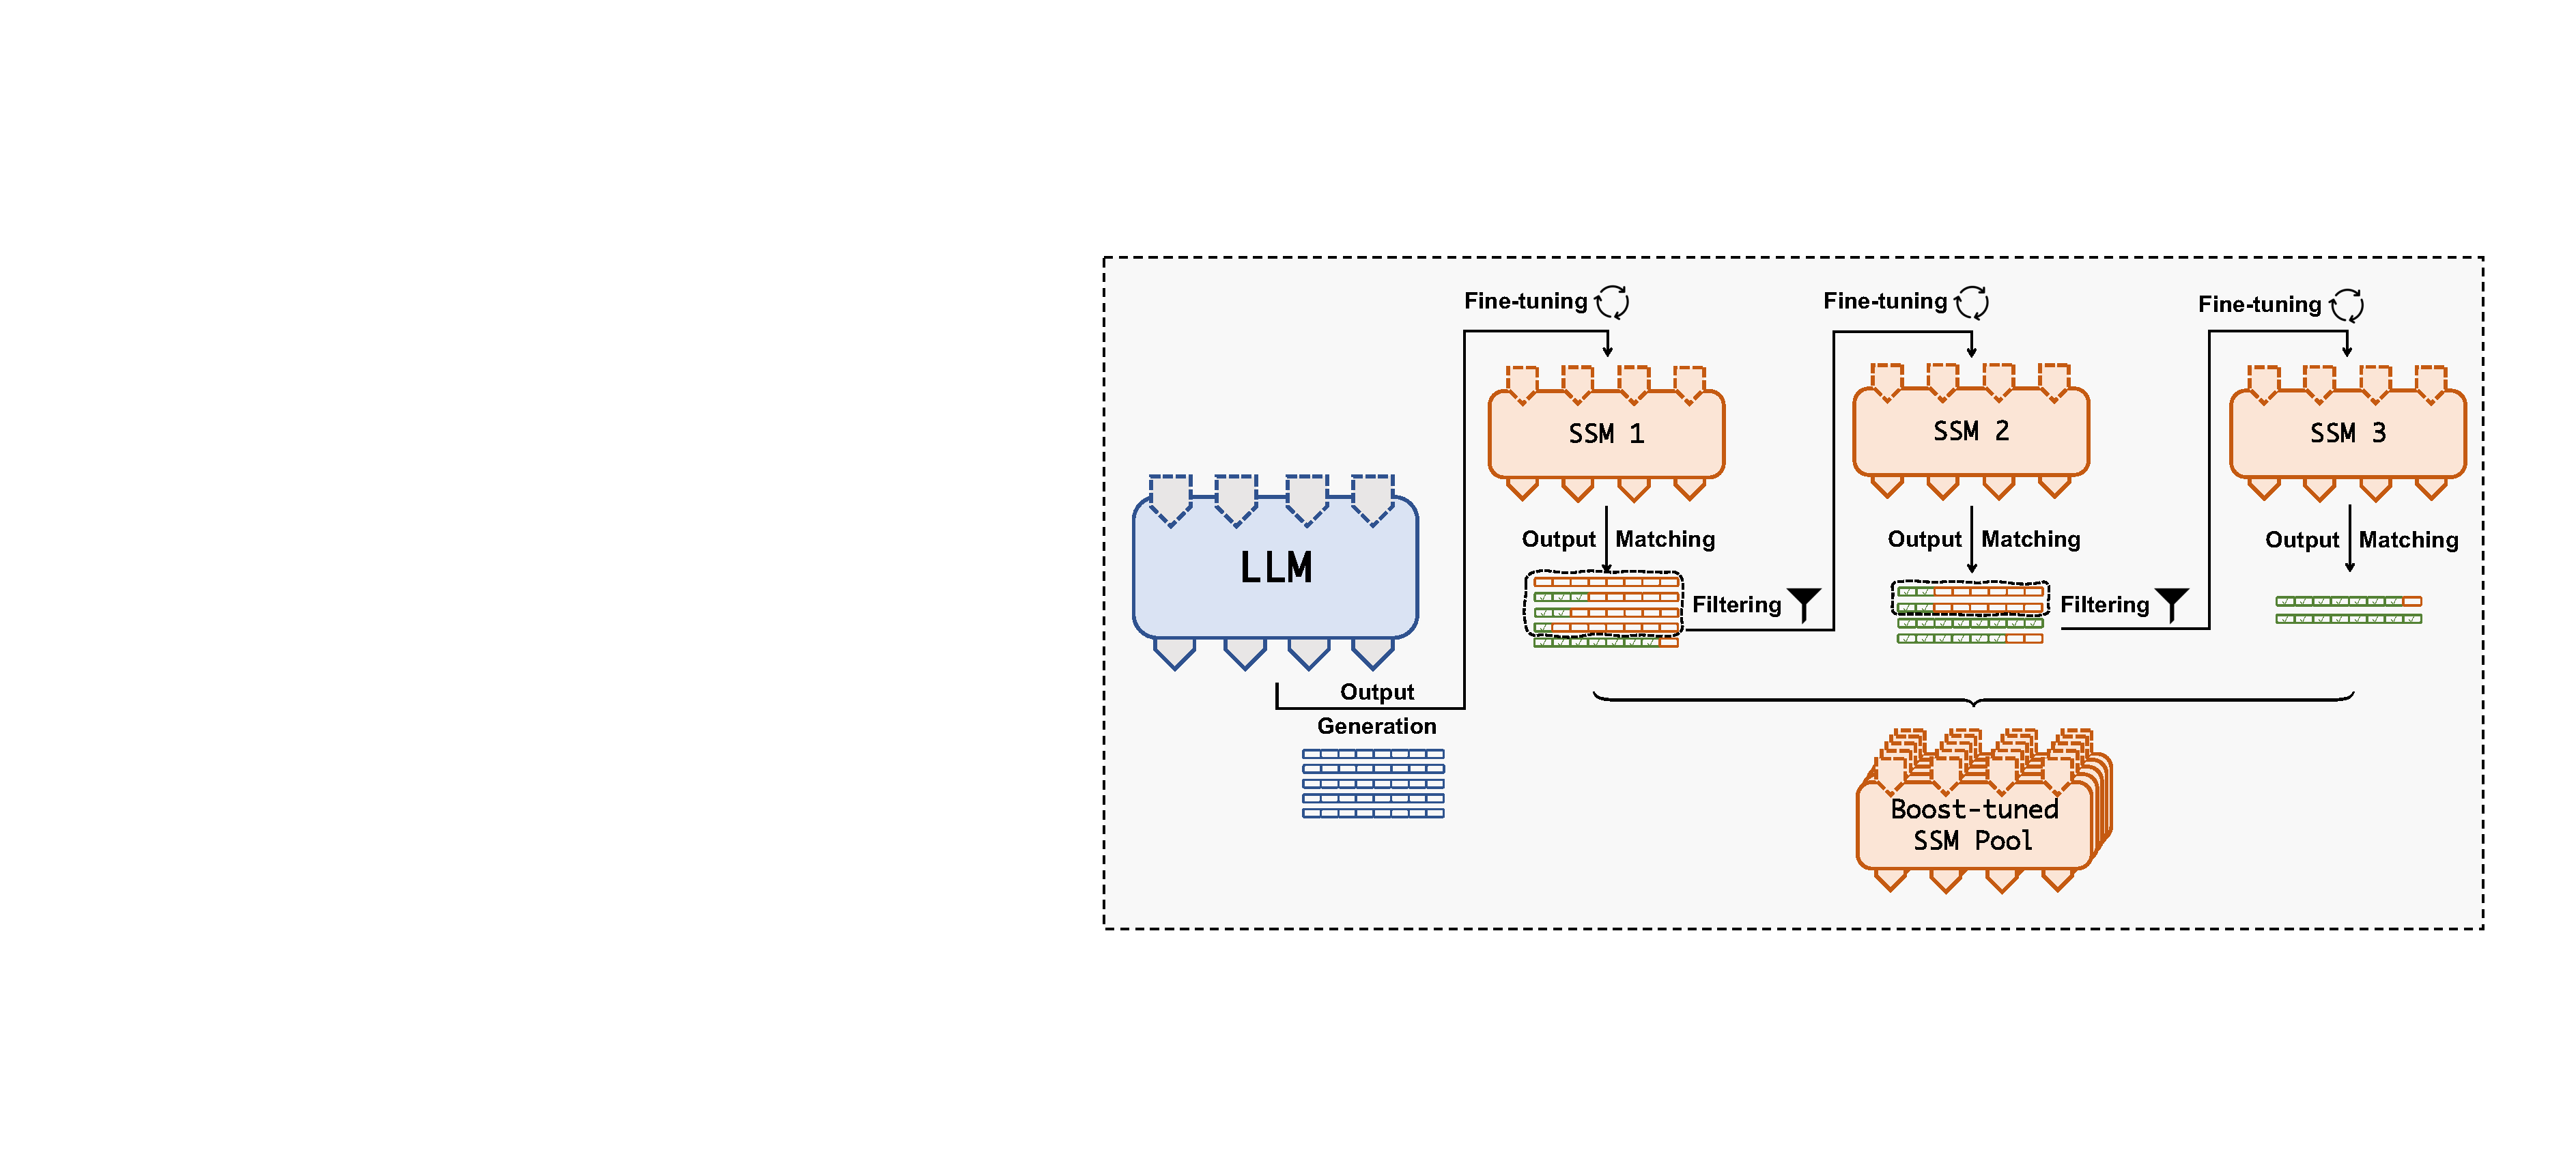
\includegraphics[scale=0.36]{figs/boost_tuning2.pdf}
    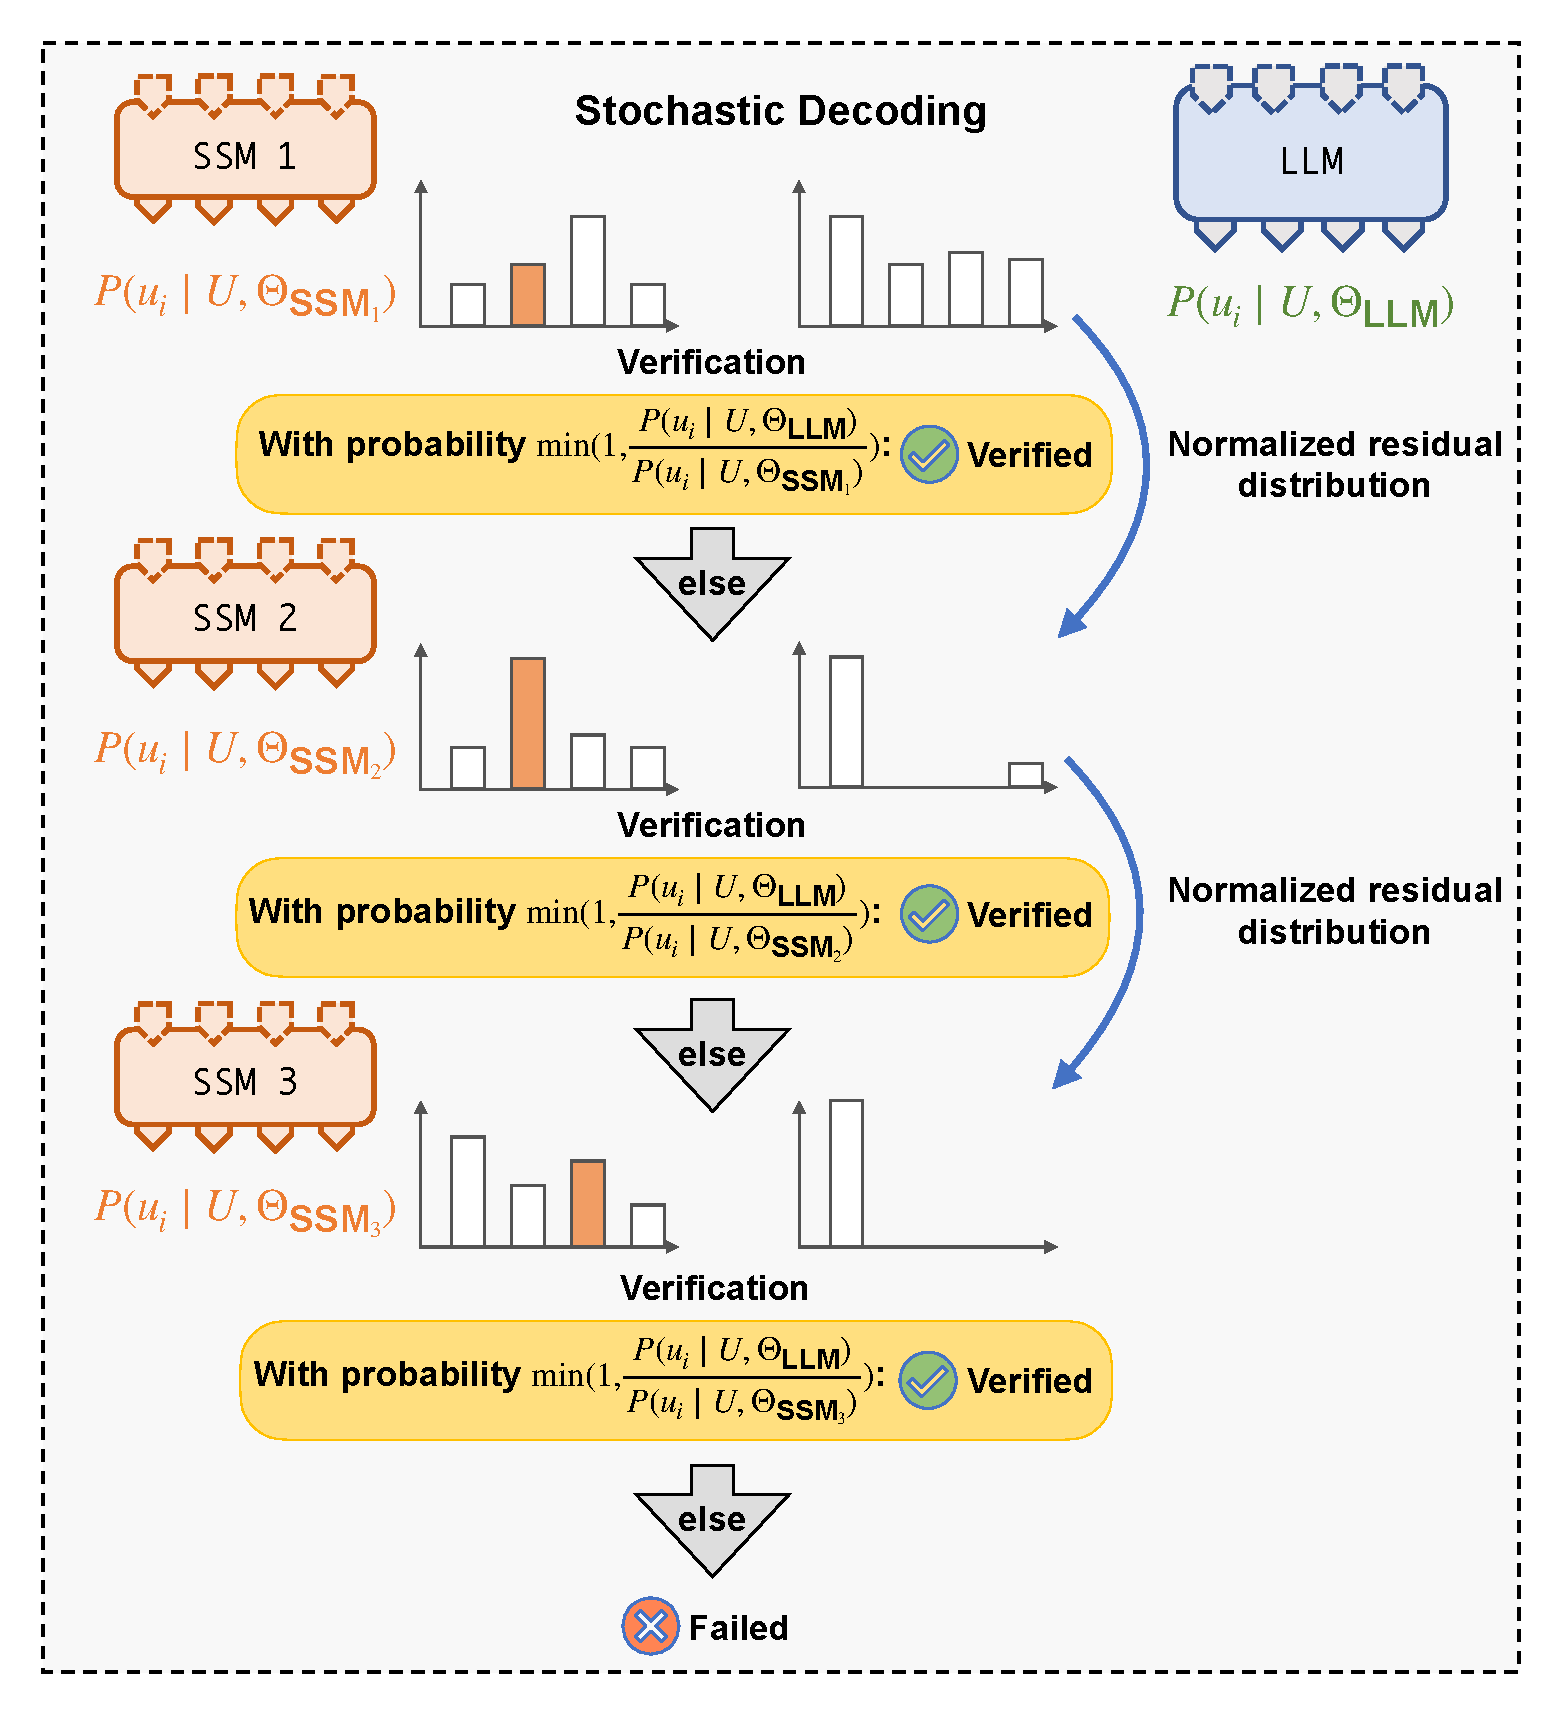
\includegraphics[scale=0.32]{figs/Decodings.pdf}
    \caption{Illustrating the multi-step speculative sampling mechanism for verifying LLMs with stochastic sampling.}
    \label{fig:decodings}
\end{figure}

\paragraph{Greedy decoding.}
Many LLM applications generate tokens using {\em greedy decoding}, which greedily selects the token with the highest likelihood in each decoding step.
The $\textproc{VerifyGreedy}$ function in \Cref{alg2} shows how \Sys verifies a speculated token tree $\m{N}$ with greedy decoding.
\Sys starts from the root of $\m{N}$ and iteratively examines a node's speculated results against the LLM's original output.
%%%
For a node $u\in\m{N}$, \Sys successfully speculates its next token if $u$ includes a child node $v$ (i.e., $p_v = u$) whose token matches the LLM's output (i.e., $t_v = \m{O}(u)$).
In this case, \Sys finishes its verification for node $u$ and moves on to examine its child $v$.
%%%
When the node $u$ does not include a child that contains the LLM's output, \Sys adds $\m{O}(u)$ as a verified node in $\m{N}$ and terminates the verification process.
%%%
Finally, all verified nodes are appended to the current generated token sequence $\m{V}$.
%%%
Token tree verification allows \Sys to opportunistically decode multiple tokens (instead of a single token in the incremental decoding approach), while preserving the same generative performance as incremental decoding.

% \begin{algorithm}
% %\small
% \caption{Generalized speculative sampling (GSS). We use $p(\cdot)$ and $q(\cdot)$ to denote the LLM's token sampling probability and SSMs' token sampling probability respectively.}
% \label{alg:gss}
% \begin{algorithmic}[1]
% \State {\bf Input:} A sequence of input tokens $\m{I}$; LLM sampling temperature $T_{L}$; SSMs sampling temperature $T_{S}$
% \State {\bf Output:} A sequence of generated tokens
% \State $\m{S} = \m{I}$
% \While{true}
% \State $\m{N}, q(\cdot \mid \m{N}/\textrm{Leaf}(\m{N})) = \Call{Speculate}{\m{S}, T_{S}}$
% \State $p(\cdot \mid \m{N}) = \Call{TreeParallelDecode}{\textrm{LLM}, \m{N}, T_{L}}$ 
% %\XM{Hhttps://www.overleaf.com/project/6400b5737cf6fcf36796d963ow about using a function that takes LLM as input to highlight the differences of using LLMs? E.g., t$\gets$Decode(LLM, S) for Algorithm 1 and $\m{O}\gets$ParallelDecode(LLM, $\m{N}$) in Algorithm 2}
% \State $\m{V} = \Call{Verify}{p, q, \m{N}}$
% \For{$t \in \m{V}$}
% \State $\m{S}$.append($t$)
% \If{$t = \langle \textrm{EOS} \rangle$}
% \State {\bf return} $\m{S}$
% \EndIf
% \EndFor
% \EndWhile
% \State
% \Function{Verify}{$p, q, \m{N}$}
% \State $\m{V} = \emptyset$
% \State $u \leftarrow$ the root of token tree $\m{N}$
% \While{$u$ is a non-leaf node}
% \LineComment{get the children nodes of $u$}
% \State $\m{H} = \textrm{child}(u)$ 
%     \While{{\bf not} is\_empty($\m{H}$)}
%     \LineComment{get $q_{i}(\cdot\mid u)$ with the smallest total variation distance w.r.t $p(\cdot\mid u)$}
%     \State $s = \arg\min_{i \in \m{H}} \textrm{TV}\left(p(\cdot\mid u), q_{i}(\cdot\mid u)\right), r \sim U(0, 1), x_s=\m{H}[s]$ 
%         \If{$r \leq \frac{p(x_s \mid u)}{q(x_s \mid u)}$}
%             \State $\m{V}$.append($x_s$)
%             \State $u = x_s$
%             \State {\bf break}
%         \Else
%             \LineComment{normalize the residual distribution between $q(x \mid u)$ and $p(x \mid u)$}
%             \State $p(x \mid u) \coloneqq \textrm{norm}(\max(0, p(x \mid u)-q(x \mid u)))$
%             \State $\m{H}.\textrm{pop}(s)$
%         \EndIf   
%     \EndWhile
% \If{is\_empty($\m{H}$)}
%     \State {\bf break}
% \EndIf
% \EndWhile
% \State $x \sim p(\cdot \mid u)$
% \State $\m{V}$.append($x$)
% \State {\bf return} $\m{V}$
% \EndFunction
% \end{algorithmic}
% \end{algorithm}

\paragraph{Stochastic decoding.}
To improve the diversity of generated tokens, many LLM applications perform {\em stochastic decoding}, which samples a token from a probability distribution $P(u_i | u_0, ..., u_{i-1}; \Theta_{LLM})$, where $U = u_0,...,u_{i-1}$ are previously generated tokens, $u_i$ is the next token to generate, and $\Theta_{LLM}$ represents a parameterized LLM.

To verify a speculated token tree with stochastic decoding, we introduce a {\em multi-step speculative sampling} (MSS) algorithm to conduct verification, whose pseudocode code is shown in the $\textproc{VerifyStochastic}$ function in \Cref{alg2} and illustrated in \Cref{fig:decodings}.
Our method provably preserves an LLM's generative performance as incremental decoding while optimizing the number of speculated tokens that can be verified.
\Cref{thm:stochastic_sampling} proves its correctness.
% \XM{TODO: do we assume only using merge-based speculator here, rather than expansion-based speculator?}
% \ZJ{It supports both}

\begin{theorem}
\label{thm:stochastic_sampling}
For a given $LLM$ and $m$ SSMs (i.e., $SSM_1$,...,$SSM_m$, let $P(u_i | U; \Theta_{LLM})$ be the probability distribution of sampling a token using stochastic decoding, where $U = u_0,...,u_{i-1}$ are previously generated tokens, $u_i$ is the next token to generate, $\Theta_{LLM}$ represents the parameterized LLM. 

Let $P_{\rm{\Sys}}(u_i | U; \Theta_{LLM}, \{\Theta_{SSM_j}\})$ be the probability distribution of sampling token $u_i$ using \Sys's multi-step speculative sampling (see the $\textproc{VerifyStochastic}$ function in \Cref{alg2}), where $\Theta_{SSM_j}$ is the $j$-th parameterized SSM. Then $ \forall U, u_i, \Theta_{LLM}, \Theta_{SSM_j}$ we have
\begin{eqnarray}
P(u_i \mid U; \Theta_{LLM}) = P_{\rm{\Sys}}(u_i \mid U; \Theta_{LLM}, \{\Theta_{SSM_j}\})
\end{eqnarray}
\end{theorem}

%we design a generalized speculative sampling procedure that guarantees the equivalency of the sampling distribution of LLM while maximizing the number of generated tokens per verification step, as shown in~\Cref{alg:gss}. We further present the equivalency proof below.
%%%
A proof of this theorem is presented in~\cite{miao2023specinfer}.
% \Cref{sec:appendix}.

\if 0
Additionally, our generalized speculative sampling procedure has a lower overall rejection probability than a naive method which simply samples from the sampling distribution of the LLM and searches for an SSM sample matching the LLM sample. The proof is presented below.
\fi

We acknowledge that a more straightforward approach to preserving the probability distribution of stochastic decoding is directly sampling the next token $x \sim P(u_i \mid U; \Theta_{LLM})$ and examining whether $x$ is a child node of $u_{i-1}$ in the speculated token tree. We call this approach {\em naive sampling} (NS) and show that \Sys's multi-step speculative sampling has a uniformly lower rejection probability than naive sampling.

\begin{theorem}
\label{theorem:MSS}
    Let $P\left(\textrm{reject} \mid \textrm{MSS}, U, \Theta_{\textrm{LLM}}, \{\Theta_{\textrm{SSM}_j}\} \right)$ denote the probability of rejecting speculation following multi-step speculative sampling with abbreviation $P(\textrm{reject}\mid \textrm{MSS})$, and $P\left(\textrm{reject} \mid \textrm{NS}, U, \Theta_{\textrm{LLM}}, \{\Theta_{\textrm{SSM}_j}\}\right)$ the probability of rejecting speculation following Naive Sampling (NS) with abbreviation $P(\textrm{reject}\mid\textrm{NS})$. Then $\forall U, \Theta_{\textrm{LLM}}, \{\Theta_{\textrm{SSM}_j}\}$, we have $$P(\textrm{reject}\mid \textrm{MSS}) \leq P(\textrm{reject}\mid\textrm{NS})$$
\end{theorem}

We present a proof of~\Cref{theorem:MSS} in~\cite{miao2023specinfer}.
%\Cref{sec:appendix}.

\if 0
\rev{Note that prior sequence-based speculative inference work has introduced the verification algorithm for a single speculative model~\cite{leviathan2022fast, chen2023accelerating} when performing stochastic sampling. Different from these approaches, \Sys leverages multiple boosted SSMs and token trees for improving speculative performance, which requires a verification algorithm that can be generalized to more than one SSM while maximizing the verification success rate. More specifically,~\cite{leviathan2022fast, chen2023accelerating} only verifies against one speculative sampling distribution per step and fails once there is a mismatch, which is not optimal when we have multiple speculative sampling distributions to verify with. As a result, \Sys presents a multi-step verification algorithm (see \textproc{VerifyStochastic} in \Cref{alg2}) that can verify against all branches of a token to maximize the success rate while preserving equivalence as incremental decoding. [5, 26]'s stochastic verification algorithms are thus a special case of \Sys's \textproc{VerifyStochastic} algorithm when there is only a single sequence of speculated tokens.  
}
\fi

\rev{Note that prior work has introduced single-step speculative sampling for sequence-based speculative inference~\cite{leviathan2022fast, chen2023accelerating}. Different from these approaches, \Sys leverages token trees for improving speculative performance, which requires a different verification algorithm. As a result, \Sys performs multi-step verification (see \textproc{VerifyStochastic} in \Cref{alg2}) across all branches of a token to maximize the success rate while preserving equivalence as incremental decoding.
The proposed MSS algorithm not only works for  merge-based method with multiple SSMs, but also supports expansion-based method with one SSM and top-$k$ sampling.
}
